\documentclass{article}
\usepackage{amsmath}
\usepackage{graphicx}
\usepackage{lettrine}
\usepackage{hyperref}
\usepackage{fix-cm}
\usepackage{lmodern}
\setlength{\parindent}{0pt}
% \setlength{\parindent}{10pt}  
% Adjusts indent size

\begin{document}

\begin{titlepage}
    \centering
    \vspace*{1cm}
    
    \Huge
    \textbf{Planes and Birds: Minimizing Energy}
    
    \vspace{0.5cm}
    
    \Large
    Author: Tao Su
    
    \vspace{0.5cm}
    
    \large
    Instructor: Dr. Reem Jaafar
    
    \vspace{1.5cm}
    
    \textit{HornorsCalc I Fall 2024 Project Final}
    
    \vfill

    \begin{figure}[h]
        \centering
        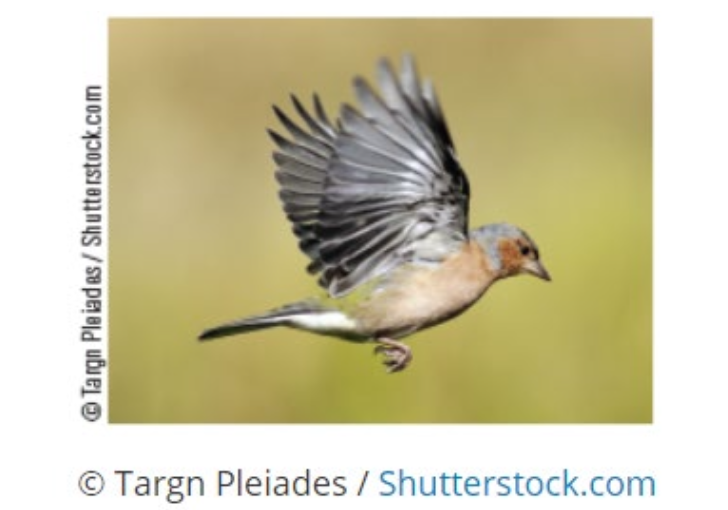
\includegraphics[width=1\textwidth]{coverPage.png}
    \end{figure}
    
    \vspace{1cm}
    \Large
    LaGuardia Community College
\end{titlepage}

\newpage

\subsection*{\itshape \large The Introduction}


{\large \lettrine[lines=2]{S}{mall} birds, like finches, alternate between flapping their wings and gliding to save energy while flying. Flapping takes a lot of power, but gliding helps conserve energy, making this pattern important for long flights. This project looks at how a bird’s flying speed affects the power it needs and the energy it uses, focusing on finding the most energy-efficient speeds.

The goal is to understand how speed influences energy use and to find the speeds where birds fly most efficiently. These ideas are similar to the way fixed-wings plane balance power and fuel efficiency. By studying birds, we can learn more about energy use in both nature and human-made systems.

In this project, we use ideas from calculus to analyze these patterns. Specifically, we use the first derivative to find points where power use is at its highest or lowest. Then, we use the second derivative to figure out whether these points represent efficient speeds or not. These concepts of optimization, covered in Chapter 4.7, help us solve problems by using math to find the optimized points in a system or vise versa.

This project fits the purpose of how calculus can solve real-world problems. By applying what we’ve learned from calculus to birds in flight, we can better understand how math explains energy use in nature. It also shows how the same tools we use in class can apply to other areas, like science and engineering.

Through this project, we hope to learn more about energy efficiency in bird flight and show how math can be used to solve practical problems.}

\newpage


\subsection*{Part 1:}
\begin{figure}[h]
    \centering
    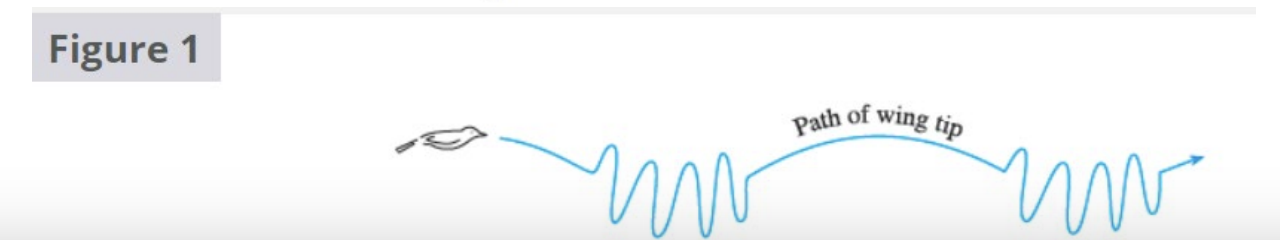
\includegraphics[width=0.5\textwidth]{bird.png}
    \caption{\small The trajectory of a flying bird.}
    \label{fig:bird}
\end{figure}

{\large \bfseries The power needed to propel an airplane forward at velocity \( v \) is: 
}\[
P = Av^3 + \frac{BL^2}{v}.
\]
{\large \bfseries where \( A \) and \( B \) are positive constants specific to the particular aircraft, and \( L \) is the lift—the upward force supporting the weight of the plane (or bird). Find the speed that minimizes the required power.}
\setlength{\parskip}{2em}

To determine the relationship between the power \(P\) and the speed \(v\), we can start with finding the derivative of \(P'\) with respect to \(v\).

The derivative of \( P \) with respect to \( v \) is:
\[
P'(v) = 3Av^2 - \frac{BL^2}{v^2}.
\]

To find the critical point of \( P(v) \), we set \( P'(v) = 0 \):
\[
P'(v) = 3Av^2 - \frac{BL^2}{v^2} = 0.
\]
Solving for \( v \), we get:
\[
v^4 = \frac{BL^2}{3A}.
\]
Therefore, we can find the speed \( V \) as:
\[
V = \sqrt[4]{\frac{BL^2}{3A}}.
\]

To determine whether this speed represents a minimum or maximum, we test the second derivative:
\[
P''(v) = 6Av + \frac{2BL^2}{v^3}.
\]

Since \( A \) and \( B \) are positive constants, and \( L^2 \) and \( v \) are always positive, we find that:
\[
P''(v) = 6Av + \frac{2BL^2}{v^3} > 0.
\]

Thus, when \( P'(v) = 0 \) and \( P''(v) > 0 \), \( P \) concaved up, indicating an absolute minimum. Therefore, when
\[
\text{the speed } V \text{ when power } p \text{ is minimized }  V_p = \sqrt[4]{\frac{BL^2}{3A}}
\]
the required power \( P \) is minimized.

\subsection*{Part 2:}
{\large \bfseries The speed found in Part 1 minimizes power, but a faster speed might use less fuel. The energy needed to propel the airplane/bird a unit distance is \( E = \frac{P}{v} \). At what speed is energy minimized?}

To find out the answer, we first need to know the relationship between \( E \) and \( v \). 

Fortunately, we know:
\[
P = Av^3 + \frac{BL^2}{v} \text{ from the beginning, and }
E = \frac{P}{v}
\]

So, we can easily derive the equation for \( E(v) \):
\[
E(v) = Av^2 + \frac{BL^2}{v^2}
\]
Next, let's take the derivative of \(E\) respect to \(v\):
\[
E'(v) = 2Av-\frac{2BL^2}{v^3}
\]
Same as part 1, we also need to find the critical point of \(E'(v)\):
\[\text{We set } E'(v) = 2Av-\frac{2BL^2}{v^3} = 0,\]
\[\text{ solve for }v, v^4=\frac{2BL^2}{2A}, v = \sqrt[4]{\frac{BL^2}{A}},\text{ and }V > 0.\]
Then we take the second derivative of \(E'\) respect to \(v\):
\[E''(v) = 2A + \frac{6BL^2}{v^4},
\text{ because } 2A > 0, \text{ and } \frac{6BL^2}{v^4} > 0, E''(v) > 0.\]
Therefore,
 \[\text{when the speed }V_e = \sqrt[4]{\frac{BL^2}{A}}, E\text{ has the absolute minimum,}\]
  the energy is minimized.

\subsection*{Part 3:}
{\large \bfseries How much faster is the speed for minimum energy than the speed for minimum power?
}\setlength{\parskip}{1em}

By observation, we found that both \(V_p\)(the speed \(V\) when power \(p\) is minimized) and \(V_e\) (the speed \(V\) when energy \(e\) is minimized) are 4th root, therefore, we can compare these two value by dividing \(V_e\) by \(V_p\):
\[\frac{V_e}{V_p}=\frac{\sqrt[4]{\frac{BL^2}{A}}}{\sqrt[4]{\frac{BL^2}{3A}}} = \sqrt[4]{3}\]

Therefore, we can conclude that, the speed \(V_e\) for minimum energy is \(\sqrt[4]{3}\) times faster than the speed for minimum power \(V_p\).

\subsection*{Part 4:}
\label{sec:part4}
{\large \bfseries In applying the equation of Part 1 to bird flight we split the term \(Av^3\)into two
parts: \(A_bv^3\) for the bird’s body and \(A_wv^3\) for its wings. Let \(x\) be the fraction of flying time spent in flapping mode. If \(m\) is the bird’s mass and all the lift occurs during flapping, then the lift is \(\frac{mg}{x}\) and so the power needed during flapping is:
\[P_\text{flap} = (A_b+A_w)v^3+\frac{B(\frac{mg}{x})^2}{v}\]
The power while wings are folded is \(P_\text{fold}=A_bv^3\). Show that the average power over an entire flight cycle is:
\[\overline{P}=xP_\text{flap}+(1-x)P_\text{fold} = A_bv^3+xA_wv^3+\frac{Bm^2g^2}{xv}\]}

To address this problem, first, let's break it down:

 The energy \(E\) for the whole cycle is actually generated by bird flapping its wings during the time of flapping stage, afterward, the bird stops flapping and folds its wings.

 But birds keeps flying, more acurately, it keeps gliding, during the time of folding stage, bird doesn't spend more energy, instead, it uses the remaining energy from the flapping stage.

Therefore, the total energy during the whole flying process is qual to the energy during flapping, and by the physics definition, the relationship between power \(P\) and energy \(E\) is:
\[\overline{P}=\frac{\Delta E}{\Delta t}\]
And the time during flapping is fraction \(x\), then the time during folding would be \(1-x\), therefore:
\[\text{the energy spends during flapping is } E_\text{flap} =P_\text{flap}\times  x \]
\[\text{the energy spends during folding is } E_\text{fold} = P_\text{fold}\times (1-x)\] 
\[\text{the total energy spent during the flying cycle would be: }E = E_\text{flap} +E_\text{fold} \]
And then,let's come back to the definition of power:
 \[\overline{P}=\frac{\Delta E}{\Delta t}=\frac{E}{x+(1-x)}=\frac{E_\text{flap}+E_\text{fold}}{1}=\frac{P_\text{flap}x + P_\text{fold}(1-x)}{1}\]
 Therefore:
\[\overline{P}=P_\text{flap}+P_\text{fold}(1-x)=((A_b+A_w)v^3+\frac{B(\frac{mg}{x})^2}{v})x+(A_bv^3)(1-x)\] 
\[= A_bv^3+xA_wv^3+\frac{Bm^2g^2}{xv}\]
Thus, we proved the hypothesis of average power during each flying cycle.


\subsection*{Part 5:}
{\large \bfseries For what value of \(x\) is the average power a minimum?
}\setlength{\parskip}{1em}

We've got the average power \(\overline{P}\) from the part 4, then let's take the derivative of \(\overline{P}\) respect to \(x\):
\[\overline{P}\text{ }'(x)= A_wv^3-\frac{Bm^2g^2}{x^2v}\]
and its second derivative:
\[\overline{P}\text{ }'' = \frac{2Bm^2g^2}{x^3v}\]
We found that, the second derivative of \(\overline{P}\) will be greater than \(0\), then we just need to find the \(x\) to make  \(\overline{P}\text{ }' = 0\):
\[\text{solve for }x \text{: }\overline{P}\text{ }'(x)= A_wv^3-\frac{Bm^2g^2}{x^2v} =0 \]
\[A_wv^3 = \frac{Bm^2g^2}{x^2v}, x = \sqrt{\frac{Bm^2g^2}{A_wv^4}} = \frac{mg}{v^2}\sqrt{\frac{B}{A_w}},\text{ and }x > 0\]
Therefore, when \(x = \frac{mg}{v^2}\sqrt{\frac{B}{A_w}}\), the average power is minimized.

\subsection*{Part 6:}
{\large \bfseries The average energy over a cycle is \(\overline{E} = \frac{\overline{P}}{v}\). What value of \(x\) minimizes \(\overline{E}\) ?}

Since we had \(\overline{P}\) from \hyperref[sec:part4]{part 4}, we can directly calculate \(\overline{E} = \frac{\overline{P}}{v}\):
\[\overline{E} = \frac{\overline{P}}{v}=  A_bv^2+xA_wv^2 + \frac{Bm^2g^2}{xv^2} \]
Then, let's take its derivative with respect to \(x\):
\[\overline{E}\text{ }' = A_wv^2-\frac{Bm^2g^2}{x^2v^2}\]

again, we need its second derivative with respect to \(x\) to determine its extremum:
\[\overline{E}\text{ }'' = \frac{2Bm^2g^2}{x^3v^2},\]
\[\text{both }Bm^2g^2 \text{ and } x^3v^2 \text{ are positive, therefore, } \overline{E} \text{ }'' > 0\]
So, when \(\overline{E}\text{ }' = 0\), \(\overline{E}\) has the absolute minimum value.

Next, we set \(\overline{E}\text{ }' = 0\), and solve for \(x\):
\[\overline{E}\text{ }' = A_wv^2-\frac{Bm^2g^2}{x^2v^2}, A_wv^2 = \frac{Bm^2g^2}{x^2v^2},\]
\[x^2=\frac{Bm^2g^2}{A_wv^4}, x = \frac{mg}{v^2}\sqrt{\frac{B}{A_w}},\text{ and }x > 0\]

Supprisingly, we got when \(x = \frac{mg}{v^2}\sqrt{\frac{B}{A_w}}\), it minimizes \(\overline{E}\), which is as the same as the value \(x\) minimizes the average power.

This is because \(\overline{P}= \frac{{\Delta \overline{E}}}{\Delta t}\), and \(\Delta t = x + (1-x) =1\), which make \(\overline{P} = \Delta \overline{E}\ = \overline{E}\).

\subsection*{Conclusion:}
{\large \bfseries Based on parts 5 and 6, what can you conclude if the bird flies slowly? What can you conclude if the bird flies faster and faster?}

We found the relationship between the flapping time \(x\) and the speed \(v\) to minimize the average power and energy from parts 5 and 6:
\[x = \frac{mg}{v^2}\sqrt{\frac{B}{A_w}}\]

When a bird has a limited amount of energy, it adjusts its speed based on its needs. To catch prey, the bird must fly faster, which increases its power output but shortens its flight cycle. After catching the prey, the bird slows down, which extends its flight cycle. If it doesn’t slow down, the bird will need to use more energy to keep flying.

This is similar to humans: when we sprint, we use a lot of energy to run faster. But when running a marathon, we slow down to conserve energy and make it to the finish line. A bird’s survival strategy is to fly quickly when necessary, like during a hunt, and slow down when it can, to save energy and stay efficient.

\textbf{\textit{But}}, the real world is far more complicated than our model, the bird's flight is influenced by many factors, such as the wind, the temperature, the humidity, and the bird's physical condition, etc. And if a bird flies too slow, it nees more energy to maintain its lift to stay aloft, if the bird flies too fast, the air resistance increases significantly, neither the extreme case is the optimal survive strategy for the bird, I really want to discuss about the optimal flying strategy, but the wisdom hides inside the body of a tiny bird is far beyond than my limit. Therefore, the bird's flight strategy is not only determined by the speed. These found make me agiain appreciate the complexity of the nature, and the beauty of the mathematics.

\end{document}